\documentclass[border=3pt,tikz]{standalone}
\usepackage{amsmath} % for aligned
\usepackage{listofitems} % for \readlist to create arrays
\usetikzlibrary{arrows.meta} % for arrow size
\usepackage[outline]{contour} % glow around text
\contourlength{1.4pt}

% COLORS
\usepackage{xcolor}
\colorlet{myred}{red!80!black}
\colorlet{myblue}{blue!80!black}
\colorlet{mygreen}{green!60!black}
\colorlet{myorange}{orange!70!red!60!black}
\colorlet{mydarkred}{red!30!black}
\colorlet{mydarkblue}{blue!40!black}
\colorlet{mydarkgreen}{green!30!black}

% STYLES
\tikzset{
  >=latex, % for default LaTeX arrow head
  node/.style={thick,circle,draw=myblue,minimum size=17,inner sep=0.5,outer sep=0.6},
  node in/.style={node,blue!20!black,draw=myblue!30!black,fill=myblue!25},
  node hidden/.style={node,red!20!black,draw=myred!30!black,fill=myred!20},
  node convol/.style={node,orange!20!black,draw=myorange!30!black,fill=myorange!20},
  node out/.style={node,red!20!black,draw=myred!30!black,fill=myred!20},
  connect/.style={thick,mydarkblue}, %,line cap=round
  connect arrow/.style={-{Latex[length=4,width=3.5]},thick,mydarkblue,shorten <=0.5,shorten >=1},
  node 1/.style={node in}, % node styles, numbered for easy mapping with \nstyle
  node 2/.style={node hidden},
  node 3/.style={node out}
}
\def\nstyle{int(\lay<\Nnodlen?min(2,\lay):3)} % map layer number onto 1, 2, or 3

\begin{document}

% NEURAL NETWORK activation
% https://www.youtube.com/watch?v=aircAruvnKk&list=PLZHQObOWTQDNU6R1_67000Dx_ZCJB-3pi&index=1

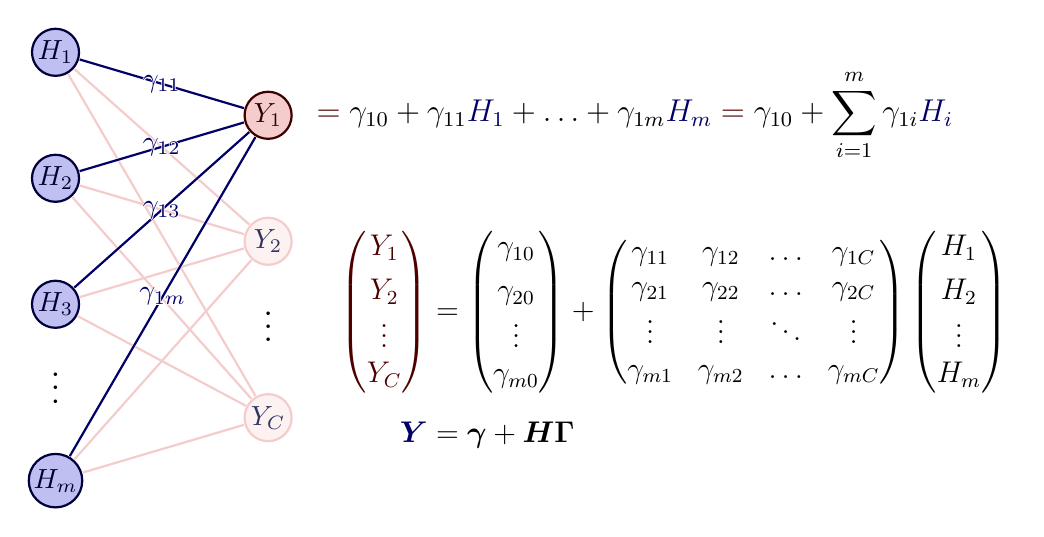
\begin{tikzpicture}[x=2.7cm,y=1.6cm]
  \message{^^JNeural network activation}
  \def\NI{4} % number of nodes in input layers
  \def\NO{3} % number of nodes in output layers
  \def\yshift{0.4} % shift last node for dots
  
  % INPUT LAYER
  \foreach \i [evaluate={\c=int(\i==\NI); \y=\NI/2-\i-\c*\yshift; \index=(\i<\NI?int(\i):"m");}]
              in {1,...,\NI}{ % loop over nodes
    \node[node in,outer sep=0.6] (NI-\i) at (0,\y) {$H_{\index}$};
  }
  
  % OUTPUT LAYER
  \foreach \i [evaluate={\c=int(\i==\NO); \y=\NO/2-\i-\c*\yshift; \index=(\i<\NO?int(\i):"C");}]
    in {\NO,...,1}{ % loop over nodes
    \ifnum\i=1 % high-lighted node
      \node[node hidden]
        (NO-\i) at (1,\y) {$Y_{\index}$};
      \foreach \j [evaluate={\index=(\j<\NI?int(\j):"m");}] in {1,...,\NI}{ % loop over nodes in previous layer
        \draw[connect,white,line width=1.2] (NI-\j) -- (NO-\i);
        \draw[connect] (NI-\j) -- (NO-\i)
          node[pos=0.50] {\contour{white}{$\gamma_{1\index}$}};
      }
    \else % other light-colored nodes
      \node[node,blue!20!black!80,draw=myred!20,fill=myred!5]
        (NO-\i) at (1,\y) {$Y_{\index}$};
      \foreach \j in {1,...,\NI}{ % loop over nodes in previous layer
        %\draw[connect,white,line width=1.2] (NI-\j) -- (NO-\i);
        \draw[connect,myred!20] (NI-\j) -- (NO-\i);
      }
    \fi
  }
  
  % DOTS
  \path (NI-\NI) --++ (0,1+\yshift) node[midway,scale=1.2] {$\vdots$};
  \path (NO-\NO) --++ (0,1+\yshift) node[midway,scale=1.2] {$\vdots$};
  
  % EQUATIONS
  \def\agr#1{{\color{mydarkblue}H_{#1}}} % green x_i^j
  \node[below=0,right=11,mydarkred,scale=0.95] at (NO-1)
    {$\large \begin{aligned} %\underset{\text{bias}}{\gamma_0}
       &= \color{mydarkred} \color{black}
            \gamma_{10} + \gamma_{11}\agr{1} + \ldots + \gamma_{1m}\agr{m} 
          \color{mydarkred} = \color{mydarkred} \color{black}
             \gamma_{10} + 
            \sum_{i=1}^{m} \gamma_{1i}\agr{i}
           \color{mydarkred}
     \end{aligned}$};
  \node[right,scale=0.9] at (1.3,-1.3)
    {$\large \begin{aligned}
      {\color{mydarkred}
      \begin{pmatrix}
        Y_{1} \\[0.3em]
        Y_{2} \\
        \vdots \\
        Y_{C}
      \end{pmatrix}}
      &=
      \color{black}
      \begin{pmatrix}
        \gamma_{10} \\[0.3em]
        \gamma_{20} \\
        \vdots \\
        \gamma_{m0}
      \end{pmatrix}
      + 
      \begin{pmatrix}
        \gamma_{11} & \gamma_{12} & \ldots & \gamma_{1C} \\
        \gamma_{21} & \gamma_{22} & \ldots & \gamma_{2C} \\
        \vdots  & \vdots  & \ddots & \vdots  \\
        \gamma_{m1} & \gamma_{m2} & \ldots & \gamma_{mC}
      \end{pmatrix}
      \begin{pmatrix}
        H_{1} \\[0.3em]
        H_{2} \\
        \vdots \\
        H_{m}
      \end{pmatrix}
      \\[0.5em]
      {\color{mydarkblue}\boldsymbol{Y}} % vector (bold)
      &= \color{mydarkred} \color{black}
           \boldsymbol{\gamma} + \boldsymbol{H}\boldsymbol{\Gamma} 
         \color{mydarkred}
    \end{aligned}$};
  
\end{tikzpicture}

\end{document}
